% !TEX program = pdflatex
\documentclass[conference]{IEEEtran}

\usepackage{amsmath,amssymb,amsfonts}
\usepackage{pifont}
\usepackage{algorithmic}
\usepackage{graphicx}
\graphicspath{{figures/}{./}}
\usepackage{textcomp}
\usepackage{xcolor}
\usepackage{cite}
\usepackage{booktabs}
\usepackage{multirow}
\usepackage{url}
\usepackage{subcaption}
\usepackage{enumitem}
\usepackage{flushend}
\setlist{noitemsep, topsep=2pt, leftmargin=*}
\setlength{\textfloatsep}{6pt plus 2pt minus 2pt}
\setlength{\floatsep}{6pt plus 2pt minus 2pt}
\setlength{\intextsep}{6pt plus 2pt minus 2pt}
\setlength{\abovecaptionskip}{3pt}
\setlength{\belowcaptionskip}{-2pt}

\def\BibTeX{{\rm B\kern-.05em{\sc i\kern-.025em b}\kern-.08em
    T\kern-.1667em\lower.7ex\hbox{E}\kern-.125emX}}

\begin{document}

\title{Fine-Grained Spiking Semantic Communication with Spatial Masking for Aerial Scene Classification}

\author{\IEEEauthorblockN{Anonymous Author(s)}
\IEEEauthorblockA{Paper ID: XXXX}}

\maketitle

\begin{abstract}
UAV edge intelligence must cope with both unreliable air-to-ground links and stringent onboard power limits. We present \textbf{SpikeAdapt-SC}, a spiking semantic communication system for aerial scene classification that combines a native $14\times14$ spatial grid, learned block masking, and low-rate spike-domain transmission. The key design choice is to avoid coarse pooling: on the native grid, masking becomes fine-grained enough to improve robustness under noise rather than merely save bandwidth. Over 5~seeds with full pipeline retraining, SpikeAdapt-SC achieves $94.86{\pm}0.63$\% (AID) and $92.52{\pm}0.17$\% (RESISC45) clean accuracy at $\rho{=}0.75$, with only $\sim$2~pp degradation at BER$=0.30$. On RESISC45, masking at $\rho{=}0.75$ significantly improves BER$=0.30$ accuracy over full-rate ($+$2.0~pp, $p{=}0.038$), while on AID masking is bandwidth-neutral. A learned-mask ablation against random and uniform masking confirms that the gain is most pronounced under harsher compression. MPBN reduces the encoder firing rate to 0.167, corresponding to 37.3$\times$ lower estimated compute energy via SynOps.
\end{abstract}

\begin{IEEEkeywords}
Semantic communication, spiking neural networks, aerial scene classification, spatial masking, energy efficiency, noisy channels
\end{IEEEkeywords}

%=====================================================================
\section{Introduction}
\label{sec:intro}
%=====================================================================

UAVs are increasingly used as mobile edge-inference platforms for scene understanding, disaster response, and environmental monitoring, but aerial semantic transmission is constrained by both unreliable air-to-ground links and strict SWaP limits on the platform itself~\cite{zeng2019uav, li2021survey, khuwaja2018survey}. Split inference is attractive for such platforms, yet transmitting intermediate features over a noisy wireless link remains costly and fragile.

Recent semantic communication (SemCom) systems show that learned feature transmission can outperform separation-based designs under adverse channels~\cite{xie2021deep, bourtsoulatze2019deep}. In parallel, SNN-based SemCom has shown that binary spikes are naturally compatible with digital links and event-driven hardware~\cite{wang2024snnsc, wang2023snnsc_harq}. However, prior SNN systems transmit all spatial locations uniformly, while adaptive-rate JSCC systems rely on ANN encoders and floating-point features~\cite{dai2022ntscc, li2024djscc}. The gap we address is a \emph{fine-grained spiking} SemCom system that can both save payload and remain robust under heavy bit errors on aerial datasets.

The central empirical finding of this paper is that \emph{granularity matters}. Coarse spatial pooling makes many blocks interchangeable; keeping the native $14\times14$ feature grid exposes a useful 196-block decision space in which learned masking becomes effective. Our contributions are:
\begin{enumerate}
    \item \textbf{Fine-grained native-grid masking.} A BER-conditioned importance scorer selects informative spatial blocks on the native $14\times14$ feature map. On RESISC45, masking at $\rho{=}0.75$ improves BER$=0.30$ accuracy by $+$2.0~pp over full-rate ($p{=}0.038$, 5-seed paired $t$-test); on AID, masking saves 25\% bandwidth with no accuracy loss under noise ($\Delta{=}-$0.20~pp, $p{=}0.69$). A controlled ablation confirms that both BER-conditioning and diversity loss are essential---removing either drops BER$=0.30$ accuracy by 20--48~pp while leaving clean accuracy unchanged. All ablation variants use the identical pipeline; only the BER branch and diversity term are toggled.
    \item \textbf{Robust spike-domain transmission.} The spiking encoder maintains high task accuracy under severe BSC corruption: over 5~seeds, accuracy degrades only $\sim$2~pp from clean to BER$=0.30$ on AID, while an 8-bit CNN baseline falls to 52.80\%.
    \item \textbf{Low-activity computation.} MPBN reduces the measured firing rate to 0.167, yielding a 37.3$\times$ SynOps energy advantage over a full-precision MAC realization under the Horowitz model~\cite{horowitz2014energy}.
\end{enumerate}

%=====================================================================
\section{Related Work}
\label{sec:related}
%=====================================================================

Deep JSCC established the value of task-oriented feature transmission under channel uncertainty~\cite{bourtsoulatze2019deep, xie2021deep}, and later work introduced spatially adaptive bit allocation for ANN-based semantic encoders~\cite{dai2022ntscc, li2024djscc}. Separately, SNN-based SemCom demonstrated that spike trains are well matched to digital transmission and can exploit event-driven computation~\cite{wang2024snnsc, wang2023snnsc_harq}. Our method combines these directions: it performs content-adaptive masking \emph{inside} an SNN split-inference pipeline for aerial scene classification, while operating on a native spatial grid rather than a pooled representation.

%=====================================================================
\section{SpikeAdapt-SC}
\label{sec:arch}
%=====================================================================

\begin{figure}[t]
    \centering
    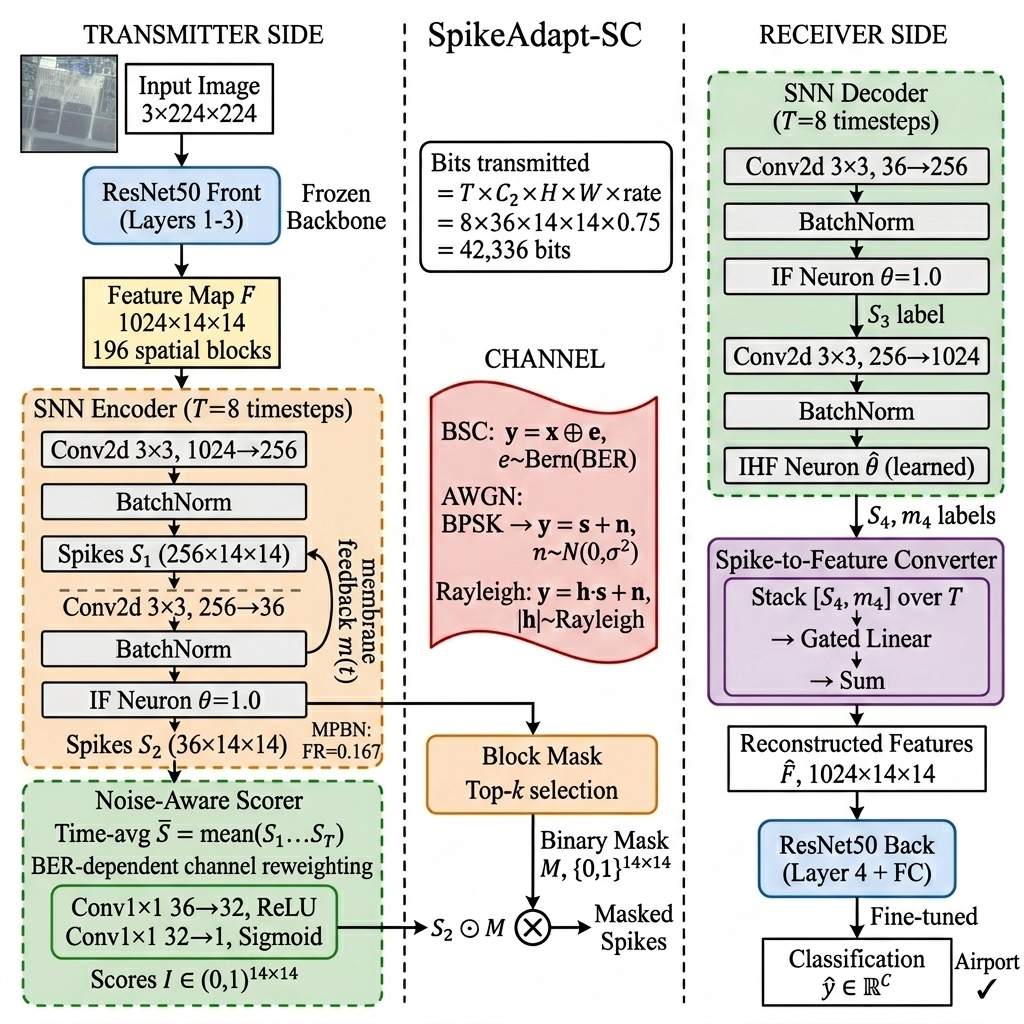
\includegraphics[width=\columnwidth]{fig1_architecture.png}
    \caption{SpikeAdapt-SC. A ResNet-50 front-end extracts $14\times14$ semantic features, an SNN encoder converts them to $T=8$ spike tensors with $C_2=36$ channels, a learned mask retains the top-$k$ spatial blocks, and the receiver reconstructs features for the ResNet back-end classifier.}
    \label{fig:architecture}
\end{figure}

A ResNet-50 front-end~\cite{he2016deep} is split at layer3, producing \(\mathbf{F}\in\mathbb{R}^{B\times 1024\times14\times14}\). Unlike earlier pooled variants, we retain this native grid to expose 196 candidate spatial blocks. The SNN encoder then maps \(\mathbf{F}\) to binary spike tensors \(\mathbf{S}_t\in\{0,1\}^{B\times36\times14\times14}\) over \(T=8\) timesteps using two 1$\times$1 convolutions, IF neurons, and MPBN~\cite{guo2023mpbn}. For layer \(l\) and timestep \(t\),
\begin{align}
    \mathbf{m}_t^{(l)} &= \mathrm{BN}_t\!\left(\mathbf{m}_{t-1}^{(l)} + \mathrm{Conv}(\mathbf{s}_t^{(l-1)})\right), \\
    \mathbf{s}_t^{(l)} &= \Theta\!\left(\mathbf{m}_t^{(l)}-v_{\text{th}}\right),\quad
    \mathbf{m}_t^{(l)} \leftarrow \mathbf{m}_t^{(l)}-\mathbf{s}_t^{(l)}v_{\text{th}},
\end{align}
with surrogate gradients for backpropagation~\cite{neftci2019surrogate}.

\subsection{BER-Conditioned Spatial Masking}

The importance scorer operates on the time-averaged spike map \(\bar{\mathbf{S}}=\frac{1}{T}\sum_t \mathbf{S}_t\). A lightweight BER branch produces per-channel reweighting,
\begin{equation}
    \mathbf{w}=1+\tanh(\mathrm{MLP}_{\text{noise}}(\mathrm{BER})),\qquad \tilde{\mathbf{S}}=\bar{\mathbf{S}}\odot \mathbf{w},
\end{equation}
followed by spatial scoring
\begin{equation}
    \mathbf{I}=\sigma\!\left(\mathrm{Conv}_{1\times1}(\mathrm{ReLU}(\mathrm{Conv}_{1\times1}(\tilde{\mathbf{S}})))+b_{\text{spatial}}(\mathrm{BER})\right).
\end{equation}
At inference, we retain the top-\(k\) entries of \(\mathbf{I}\), where \(k=\lfloor \rho HW\rfloor\). During training, a Gumbel-Softmax relaxation~\cite{jang2017categorical} enables gradient flow through the discrete mask. The loss is
\begin{equation}
\mathcal{L}=\mathcal{L}_{\text{CE}}+\lambda_{\text{rate}}(\bar{\rho}-\rho_{\text{target}})^2+\lambda_{\text{div}}\mathcal{L}_{\text{div}},
\end{equation}
where \(\mathcal{L}_{\text{div}}\) encourages clean and noisy masks to differ. This makes the scorer adapt its selection policy as BER rises, rather than converging to a single static mask.

\subsection{Bandwidth and Energy}

The transmitted payload is
\begin{equation}
    B_{\text{tx}} = \rho\,T\,C_2\,H\,W \;\text{bits}.
\end{equation}
With \(T=8\), \(C_2=36\), and \(H=W=14\), \(\rho=0.75\) corresponds to 42,336 bits per image versus 56,448 bits at full rate. On the final model, MPBN reduces firing rate from 0.266 to 0.167. Using the Horowitz model (4.6 pJ/MAC, 0.9 pJ/SynOp), this yields 201.5M SynOps and a 37.3$\times$ energy ratio at \(\rho=0.75\)~\cite{horowitz2014energy}. These are estimated compute savings, not hardware measurements.

%=====================================================================
\section{Experiments}
\label{sec:eval}
%=====================================================================

\subsection{Setup}

We evaluate on AID~\cite{xia2017aid} (10,000 images, 30 classes, 50/50 split) and NWPU-RESISC45~\cite{cheng2017resisc} (31,500 images, 45 classes, 20\% training split). The ResNet-50 backbone is ImageNet-initialized and fine-tuned first; the SNN encoder/decoder is then trained for 60 epochs, followed by 40 epochs of joint fine-tuning with the scorer and diversity loss. BSC noise is sampled during training with a high-noise-biased curriculum. Unless noted otherwise, evaluations average over three noise draws. We report 5-seed reproducibility (seeds 42, 123, 456, 789, 1024): at $\rho{=}1.0$, AID gives 95.48$\pm$0.30\% clean, 92.87$\pm$1.19\% at BER$=$0.30; RESISC45 gives 92.49$\pm$0.16\% clean, 83.55$\pm$6.88\% at BER$=$0.30.

We compare against a no-mask SNN baseline with the same backbone and bottleneck, plus an 8-bit CNN baseline (CNN-Uni) with matched backbone and BSC transmission. Extended CNN/MLP/JPEG sweeps are maintained in the repository but omitted here for space.

\subsection{Main Results}

\begin{table}[t]
\renewcommand{\arraystretch}{1.12}
\centering
\caption{Main BSC results. Rows with $\pm$ report 5-seed mean$\pm$std (seeds 42, 123, 456, 789, 1024). Remaining rows are seed-42.}
\label{tab:main_results}
\setlength{\tabcolsep}{4pt}
\begin{tabular}{l cc cc c}
\toprule
\multirow{2}{*}{\textbf{Method}} & \multicolumn{2}{c}{\textbf{AID}} & \multicolumn{2}{c}{\textbf{RESISC45}} & \multirow{2}{*}{\textbf{Rate}} \\
& Clean & BER=0.30 & Clean & BER=0.30 & \\
\midrule
\textbf{SpikeAdapt-SC} ($\rho{=}0.75$) & 94.86{\scriptsize$\pm$0.63} & 92.66{\scriptsize$\pm$0.95} & 92.52{\scriptsize$\pm$0.17} & \textbf{85.55}{\scriptsize$\pm$5.53} & 75\% \\
SpikeAdapt-SC ($\rho{=}0.625$)$^\dagger$ & 95.40 & 93.38 & 91.06 & \textbf{86.48} & 62.5\% \\
SNN (no mask, $\rho{=}1.0$) & \textbf{95.48}{\scriptsize$\pm$0.30} & \textbf{92.87}{\scriptsize$\pm$1.19} & 92.49{\scriptsize$\pm$0.16} & 83.55{\scriptsize$\pm$6.88} & 100\% \\
CNN-1bit (STE, $T{=}1$)$^\dagger$ & 95.32 & 87.56 & 91.48 & 85.19 & 100\% \\
CNN-Uni (8-bit)$^\dagger$ & 91.78 & 52.80 & 78.32 & 49.32 & 100\% \\
\bottomrule
\multicolumn{6}{l}{\scriptsize $^\dagger$Seed-42 only.}
\end{tabular}
\end{table}

Table~\ref{tab:main_results} shows three key outcomes. First, the spiking pipeline remains robust at BER$=0.30$: on AID, SpikeAdapt-SC drops only 2~pp from clean to BER$=0.30$, while CNN-Uni drops 39~pp. Second, spatial masking provides a significant benefit on harder tasks: on RESISC45, $\rho{=}0.75$ improves BER$=0.30$ accuracy by $+$1.99~pp over $\rho{=}1.0$ ($p{=}0.038$, 5-seed paired $t$-test). On AID, the masking effect is neutral ($\Delta{=}-$0.20~pp, $p{=}0.69$), consistent with the easier 30-class task having more spatial redundancy. The learned mask advantage grows at more aggressive compression: at $\rho{=}0.10$, learned masks outperform random by +40~pp under BER$=0.30$ (see repo). Third, a matched-payload non-spiking 1-bit CNN (CNN-1bit) achieves nearly identical clean accuracy but drops to 87.56\% on AID at BER$=0.30$---a 5.78~pp gap vs.\ SpikeAdapt-SC's 93.38\%. This confirms that the robustness advantage is not explained by binary transmission alone; temporal spike coding with $T{=}8$ timesteps provides significantly better noise resilience than single-shot binarization.

\begin{table}[t]
\renewcommand{\arraystretch}{1.12}
\centering
\caption{Learned-mask sanity check on AID. Random is averaged over 50 independent draws.}
\label{tab:mask_compare}
\begin{tabular}{c c ccc c}
\toprule
$\rho$ & BER & \textbf{Learned} & \textbf{Random} & \textbf{Uniform} & $\Delta_{\text{rand}}$ \\
\midrule
0.50 & 0.00 & 95.02 & 95.28{\scriptsize$\pm$0.12} & 90.58 & -0.26 \\
0.50 & 0.30 & \textbf{93.44} & 91.95{\scriptsize$\pm$0.15} & 85.54 & +\textbf{1.49} \\
\midrule
0.75 & 0.00 & 95.42 & 95.35{\scriptsize$\pm$0.10} & 94.70 & +0.07 \\
0.75 & 0.30 & \textbf{93.26} & 93.25{\scriptsize$\pm$0.13} & 91.78 & +\textbf{0.01} \\
\bottomrule
\end{tabular}
\end{table}

Table~\ref{tab:mask_compare} clarifies the masking mechanism. At moderate pruning (\(\rho=0.75\)), learned and random masks are nearly tied, which is consistent with residual spatial redundancy on aerial scene features. At more aggressive pruning (\(\rho=0.50\)), the learned scorer gains 1.49 pp over random at BER$=0.30$ and substantially exceeds the fixed uniform mask. This is the core evidence that the scorer is learning a useful selection policy rather than benefiting from pruning alone.

\begin{figure}[t]
    \centering
    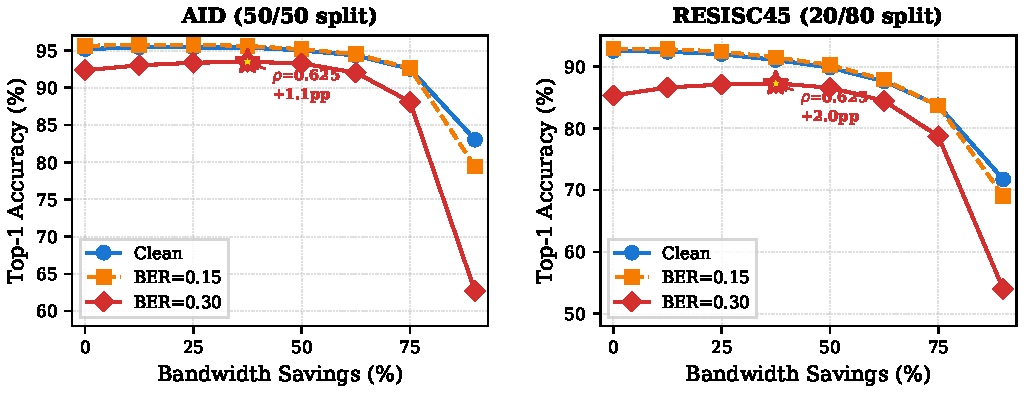
\includegraphics[width=\columnwidth]{fig5_rho_sweep_pareto.pdf}
    \caption{Rate--accuracy tradeoff on AID and RESISC45. Under severe noise, $\rho=0.625$ (37.5\% bandwidth savings) matches or exceeds full-rate $\rho=1.0$ on RESISC45; on AID the masking benefit is seed-dependent.}
    \label{fig:pareto}
\end{figure}

Fig.~\ref{fig:pareto} shows the full rate--accuracy curve. Accuracy degrades gracefully from \(\rho=1.0\) to \(\rho=0.625\), then falls more quickly at lower rates. The curve is important because it shows that the best noisy operating point is not the full-rate setting; masking creates a usable Pareto frontier rather than a monotonic compression penalty.

\subsection{Noise-Aware Ablation}

To validate that both the BER-conditioning branch and the diversity loss are essential, we retrain the S3 scorer under four configurations from the same S2-pretrained encoder/decoder (Table~\ref{tab:na_ablation}). On both datasets, the full model retains $>$87\% at BER$=0.30$, while removing either component causes a catastrophic drop: on RESISC45, all ablated variants collapse to $\sim$40\% (vs.\ 87.10\%), and on AID to $\sim$72\% (vs.\ 93.40\%). The clean accuracy is nearly identical across variants, confirming that the noise-aware machinery sacrifices no clean performance.

\begin{table}[t]
\renewcommand{\arraystretch}{1.12}
\centering
\caption{Noise-aware ablation. Both BER-conditioning and diversity loss are essential for noise robustness.}
\label{tab:na_ablation}
\setlength{\tabcolsep}{3pt}
\begin{tabular}{l cc cc cc}
\toprule
& \multicolumn{2}{c}{\textbf{Component}} & \multicolumn{2}{c}{\textbf{AID}} & \multicolumn{2}{c}{\textbf{RESISC45}} \\
\textbf{Variant} & BER & Div & Clean & 0.30 & Clean & 0.30 \\
\midrule
Full & \ding{51} & \ding{51} & 95.42 & \textbf{93.40} & 92.01 & \textbf{87.10} \\
No BER & \ding{55} & \ding{51} & 95.66 & 72.56 & 92.27 & 41.52 \\
No Div & \ding{51} & \ding{55} & 95.82 & 72.42 & 92.35 & 42.83 \\
Neither & \ding{55} & \ding{55} & 95.72 & 72.32 & 92.18 & 39.46 \\
\bottomrule
\end{tabular}
\end{table}

%=====================================================================
\section{Conclusion}
\label{sec:conclusion}
%=====================================================================

SpikeAdapt-SC shows that fine-grained masking and spike-domain transmission are complementary for aerial semantic communication. The native $14\times14$ grid makes learned masking effective; the spiking bottleneck remains robust under severe bit errors; and MPBN lowers spike activity enough to provide large estimated compute savings. A controlled ablation confirms that both BER-conditioning and diversity loss are essential---removing either collapses noise robustness by 20--48~pp while leaving clean accuracy unchanged; all variants use the identical pipeline with only the BER branch and diversity term toggled. A matched-payload non-spiking 1-bit baseline demonstrates that the robustness advantage is not explained by binary transmission alone; temporal spike coding provides 5.78~pp additional resilience at BER$=0.30$ on AID. On RESISC45, masking at $\rho{=}0.75$ significantly improves BER$=0.30$ accuracy ($+$2.0~pp, $p{=}0.038$); on AID, reduced-rate masking can match or slightly exceed full-rate performance under severe noise in some settings while remaining competitive overall.

%=====================================================================
% REFERENCES
%=====================================================================
\bibliographystyle{IEEEtran}

\begin{thebibliography}{16}

\bibitem{zeng2019uav}
Y.~Zeng, Q.~Wu, and R.~Zhang, ``Accessing from the sky: A tutorial on UAV communications for 5G and beyond,'' \emph{Proc. IEEE}, vol.~107, no.~12, pp.~2327--2375, 2019.

\bibitem{li2021survey}
B.~Li, Z.~Fei, and Y.~Zhang, ``UAV communications for 5G and beyond,'' \emph{IEEE Access}, vol.~7, pp.~36717--36732, 2019.

\bibitem{khuwaja2018survey}
A.~A.~Khuwaja \emph{et al.}, ``A survey of channel modeling for UAV communications,'' \emph{IEEE Commun. Surveys Tuts.}, vol.~20, no.~4, pp.~2804--2830, 2018.

\bibitem{xie2021deep}
H.~Xie, Z.~Qin, G.~Y.~Li, and B.-H.~Juang, ``Deep learning enabled semantic communication systems,'' \emph{IEEE Trans. Signal Process.}, vol.~69, pp.~2663--2675, 2021.

\bibitem{bourtsoulatze2019deep}
E.~Bourtsoulatze, D.~B.~Kurka, and D.~G\"{u}nd\"{u}z, ``Deep joint source-channel coding for wireless image transmission,'' \emph{IEEE Trans. Cogn. Commun. Netw.}, vol.~5, no.~3, pp.~567--579, 2019.

\bibitem{wang2024snnsc}
M.~Wang, J.~Li, M.~Ma, and X.~Fan, ``SNN-SC: A spiking semantic communication framework for collaborative intelligence,'' \emph{IEEE Trans. Cogn. Commun. Netw.}, vol.~10, no.~5, pp.~1816--1829, 2024.

\bibitem{wang2023snnsc_harq}
M.~Wang, J.~Li, M.~Ma, and X.~Fan, ``Spiking semantic communication for feature transmission with HARQ,'' \emph{IEEE Trans. Veh. Technol.}, vol.~74, no.~6, pp.~1--13, 2025.

\bibitem{dai2022ntscc}
J.~Dai \emph{et al.}, ``Nonlinear transform source-channel coding for semantic communications,'' \emph{IEEE J. Sel. Areas Commun.}, vol.~40, no.~8, pp.~2300--2316, 2022.

\bibitem{li2024djscc}
Y.~Li, X.~Chen, X.~Deng, and J.~Gui, ``Content adaptive distributed joint source-channel coding for image transmission with hyperprior,'' \emph{IEEE Trans. Commun.}, vol.~72, no.~7, pp.~4192--4205, 2024.

\bibitem{horowitz2014energy}
M.~Horowitz, ``1.1 computing's energy problem (and what we can do about it),'' in \emph{Proc. IEEE ISSCC}, 2014, pp.~10--14.

\bibitem{neftci2019surrogate}
E.~O.~Neftci, H.~Mostafa, and F.~Zenke, ``Surrogate gradient learning in spiking neural networks,'' \emph{IEEE Signal Process. Mag.}, vol.~36, no.~6, pp.~51--63, 2019.

\bibitem{he2016deep}
K.~He, X.~Zhang, S.~Ren, and J.~Sun, ``Deep residual learning for image recognition,'' in \emph{Proc. IEEE CVPR}, 2016, pp.~770--778.

\bibitem{jang2017categorical}
E.~Jang, S.~Gu, and B.~Poole, ``Categorical reparameterization with Gumbel-Softmax,'' in \emph{Proc. ICLR}, 2017.

\bibitem{xia2017aid}
G.-S.~Xia \emph{et al.}, ``AID: A benchmark data set for performance evaluation of aerial scene classification,'' \emph{IEEE Trans. Geosci. Remote Sens.}, vol.~55, no.~7, pp.~3965--3981, 2017.

\bibitem{cheng2017resisc}
G.~Cheng, J.~Han, and X.~Lu, ``Remote sensing image scene classification: Benchmark and state of the art,'' \emph{Proc. IEEE}, vol.~105, no.~10, pp.~1865--1883, 2017.

\bibitem{davies2018loihi}
M.~Davies \emph{et al.}, ``Loihi: A neuromorphic manycore processor with on-chip learning,'' \emph{IEEE Micro}, vol.~38, no.~1, pp.~82--99, 2018.

\bibitem{guo2023mpbn}
Y.~Guo \emph{et al.}, ``Membrane potential batch normalization for spiking neural networks,'' in \emph{Proc. IEEE/CVF ICCV}, 2023, pp.~19420--19430.

\end{thebibliography}

\end{document}
